\section{Case Studies}

\begin{figure*}[!ht]
\centering
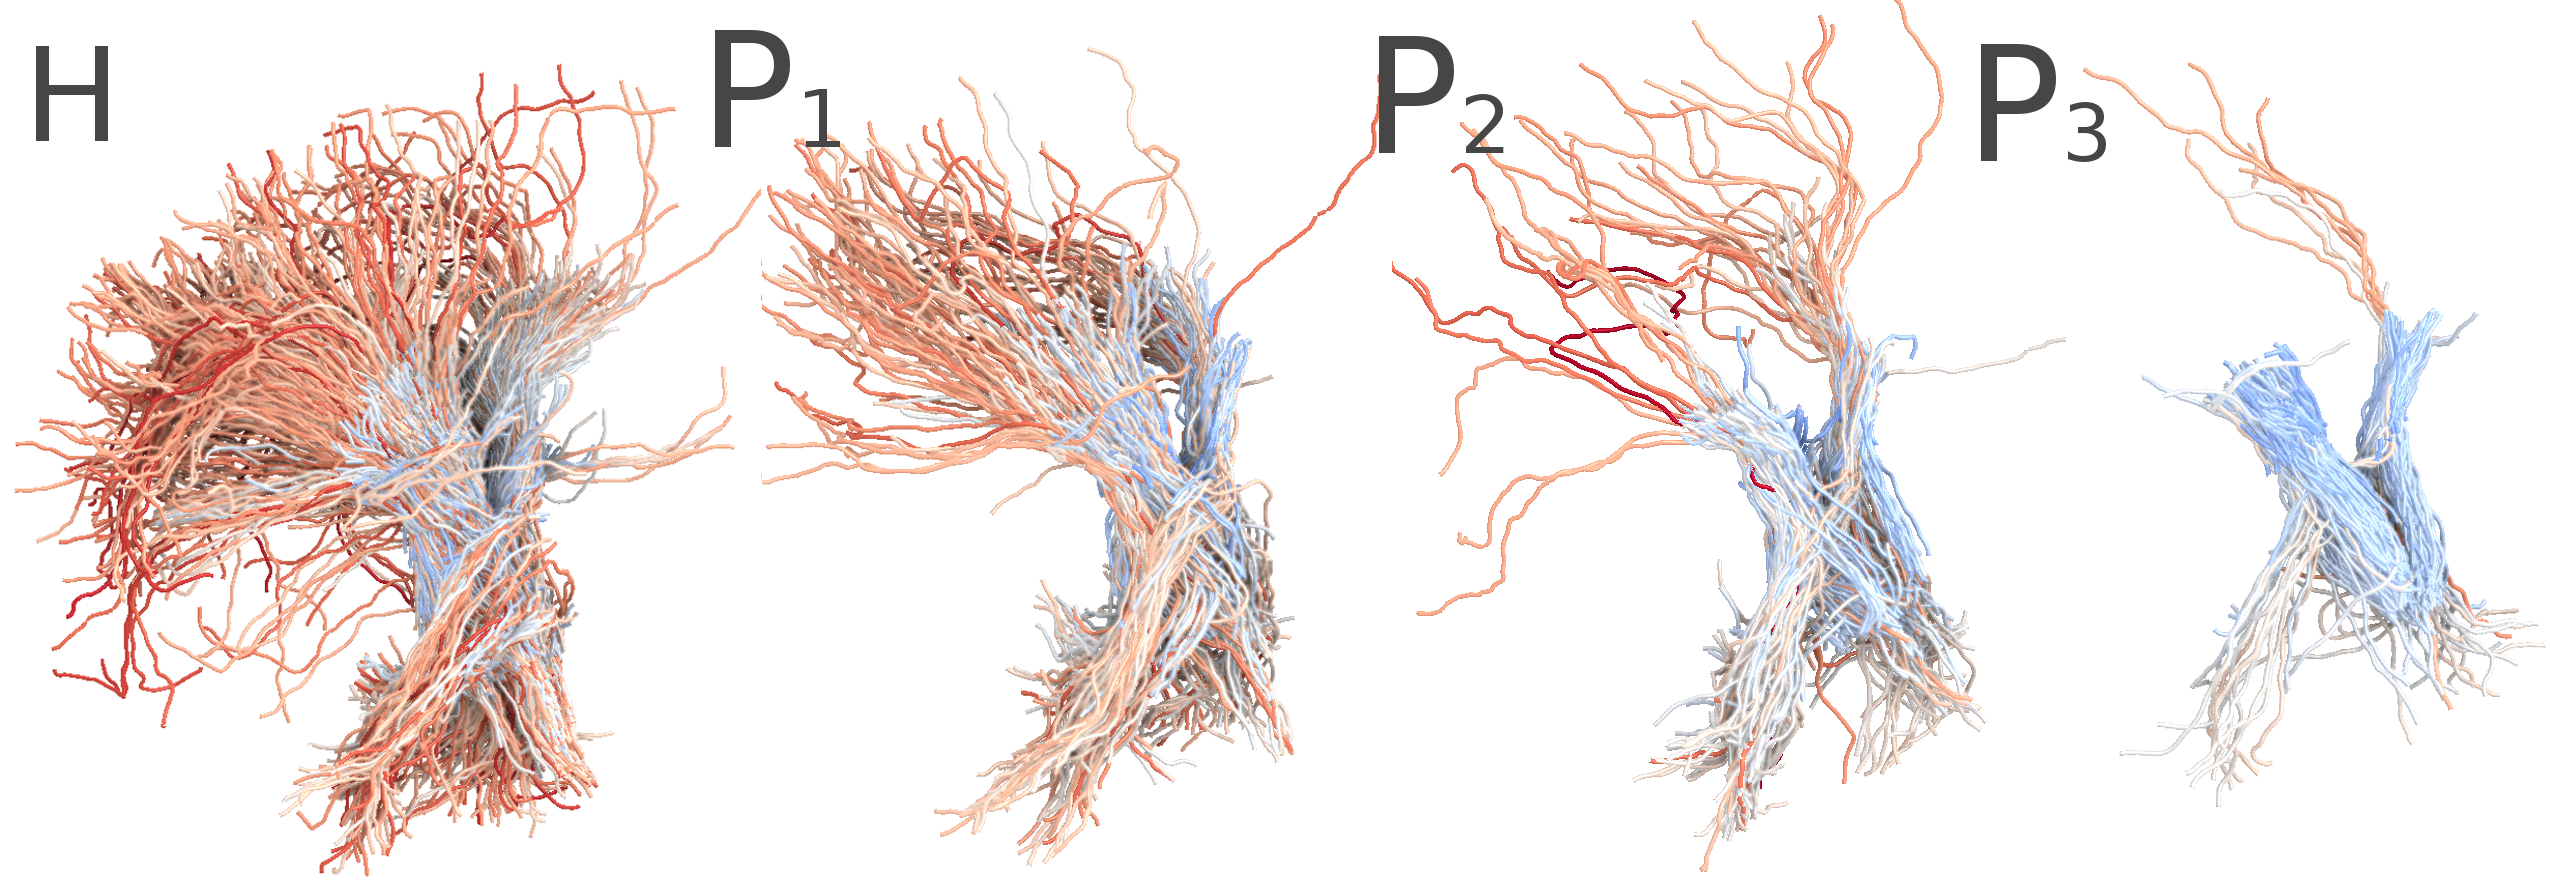
\includegraphics[width=1.0\textwidth]{degeneration.png}
\caption{The type and severity of fiber loss found among some of the disease group subjects. On the left $(H)$ shows a typical full intact region from a control group subject. $P_1$ through $P_2$ show progressively worse cases of fiber loss. This is a characteristic observed within the disease group, but the severity depicted in $P_2$ and $P_3$ were quite rare, and some apparent loss was observed within control group subjects as well.}
\label{fig:loss}
\end{figure*}

Each of our studies are based on DTI images and reconstructed fiber tracts from Parkinson's and Control groups obtained from the research database of Parkinson's Progression Markers Initiative (PPMI).  

\subsection{MRI Acquisition}

MRI scan parameters, such as gradient directions, b-value and voxel resolution, have a crucial impact on the scanned DTI images, as they provide important outcome scalar measurements that are usually the focus of clinical diagnosis study. To overcome the erroneous caused by scanners and the scan parameters, standardized acquisition protocols are very necessary. We obtained the MRI image from PPMI, where the MRI images were taken using a standardized and strict acquisition protocols developed by the steering committee on 3T Siemens scanners.

Each subject that we obtained includes DTI images and T1-weighted images. For each DTI image, a 2D echo-planar DTI sequence was acquired using the following parameters: $ TR/TE = 900/88ms$, Image matrix $= 116\times116\times72$ and voxel resolution $ = 1.98\times1.98\times2mm^3$, 64 gradient volumes (b = $1000s/mm^2$), and one non-gradient volume (b = $0s/mm^2$).  The acquisition parameters for T1-weighted images were as follows:$ TR = 2300ms, TE = 2.98ms$, Image matrix $= 160\times240\times256$ and voxel resolution $ = 1\times1\times1mm^3$. 


\subsection{DTI and T1 Preprocessing}

Both the DTI and T1 images require preprocessing. In the acquisition of diffusion images, there are variety of issues that will affect fiber tracking result, such as image intensity loss, image blurring, gradient distoration and inhomogeneities in the applied magnetic field. Without correcting MRI images, we cannot estimate fiber orientations and do fiber tracking correctly, also, we are not able to achieve alignment between DWIs and T1 images, which will affect the MRI coregistration (intra-subject registration) and finally cause great deviation of extracting fibers from Region of Interest(ROI).

All DTI and T1 images were converted from the Digital Image and Communications in Medicine (DICOM) format to Neuroimaging Informatics Technology Initiative (NIFTI) format. DTI images were preprocessed using MRtrix3 \footnote{www.mrtrix.org/}. We first denoise each DWI data, then perform Echo-planar Image (EPI)/fieldmap correction, eddy current correction and head motion correction, finally, we performed B1 field inhomogeneity correction for DWI volume series. The preprocessing procedures for T1 images are based on FreeSurfer\footnote{https://surfer.nmr.mgh.harvard.edu/}, including motion correction and non-uniformity in MR data. DWI image volumes were registered to the corresponding T1 images using FSL 5.0.10\footnote{https://fsl.fmrib.ox.ac.uk/fsl}.

\subsection{Effects of Parkinson's Disease on the Substantia Nigra Brain Region}

In this case study, we performed an analysis of the Substantia Nigra region, an important region of study in the medical literature concerning Parkinson's and other neurodegenerative diseases.

\subsubsection{Background}

Parkinson's Disease is a neurodegenerative disorder characterized by the loss of dopamine neurons in the substantia nigra (SN) brain region \cite{prakash2012asymmetrical}. The dopaminergic function of the nigrostriatal pathway will reduce with the depletion of these neurons, as well as the neural fibers that link the substantia nigra to other subcortical regions, such as putamen and caudate \cite{zhang2015diffusion}.

Each region in the mid brain is affected based on the anatomical correlation with SN and the severity of the region reflected by the functional relationship with SN\cite{zeighami2015network}. It is recognized to be a brain-wide neurodegenerative process that spreads up from brainstem into cortex, as originally suggested by Braak \cite{yau2018network}. Significant effects were also observed in the whole Parkinson's disease brain with spatial distribution of quantitative susceptibility mapping (QSM) \cite{atkinson2017diffusion}. Upon the fibers in brain are detected by tractography, it is useful to assess the diagnosis with the brain fiber pathways. 

\begin{figure}[!ht]
\centering
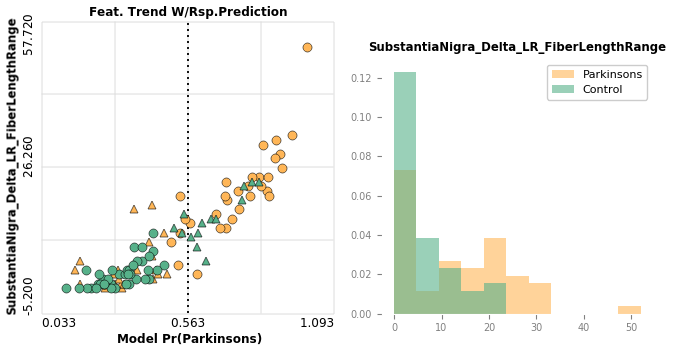
\includegraphics[width=0.5\textwidth]{DSFL.png}
\caption{Comparing the distributions of the ``Delta-Left-Right Sum of Fiber Lengths" feature (absolute difference in sum of fiber lengths between the left and right hemispheres) between the control group (blue-green) and disease group (orange). Many more subjects from the disease group are within the higher range in the feature value, yet many disease group subjects have small differences from the control group.}
\label{fig:DSFL}
\end{figure}

\begin{figure}[!ht]
\centering
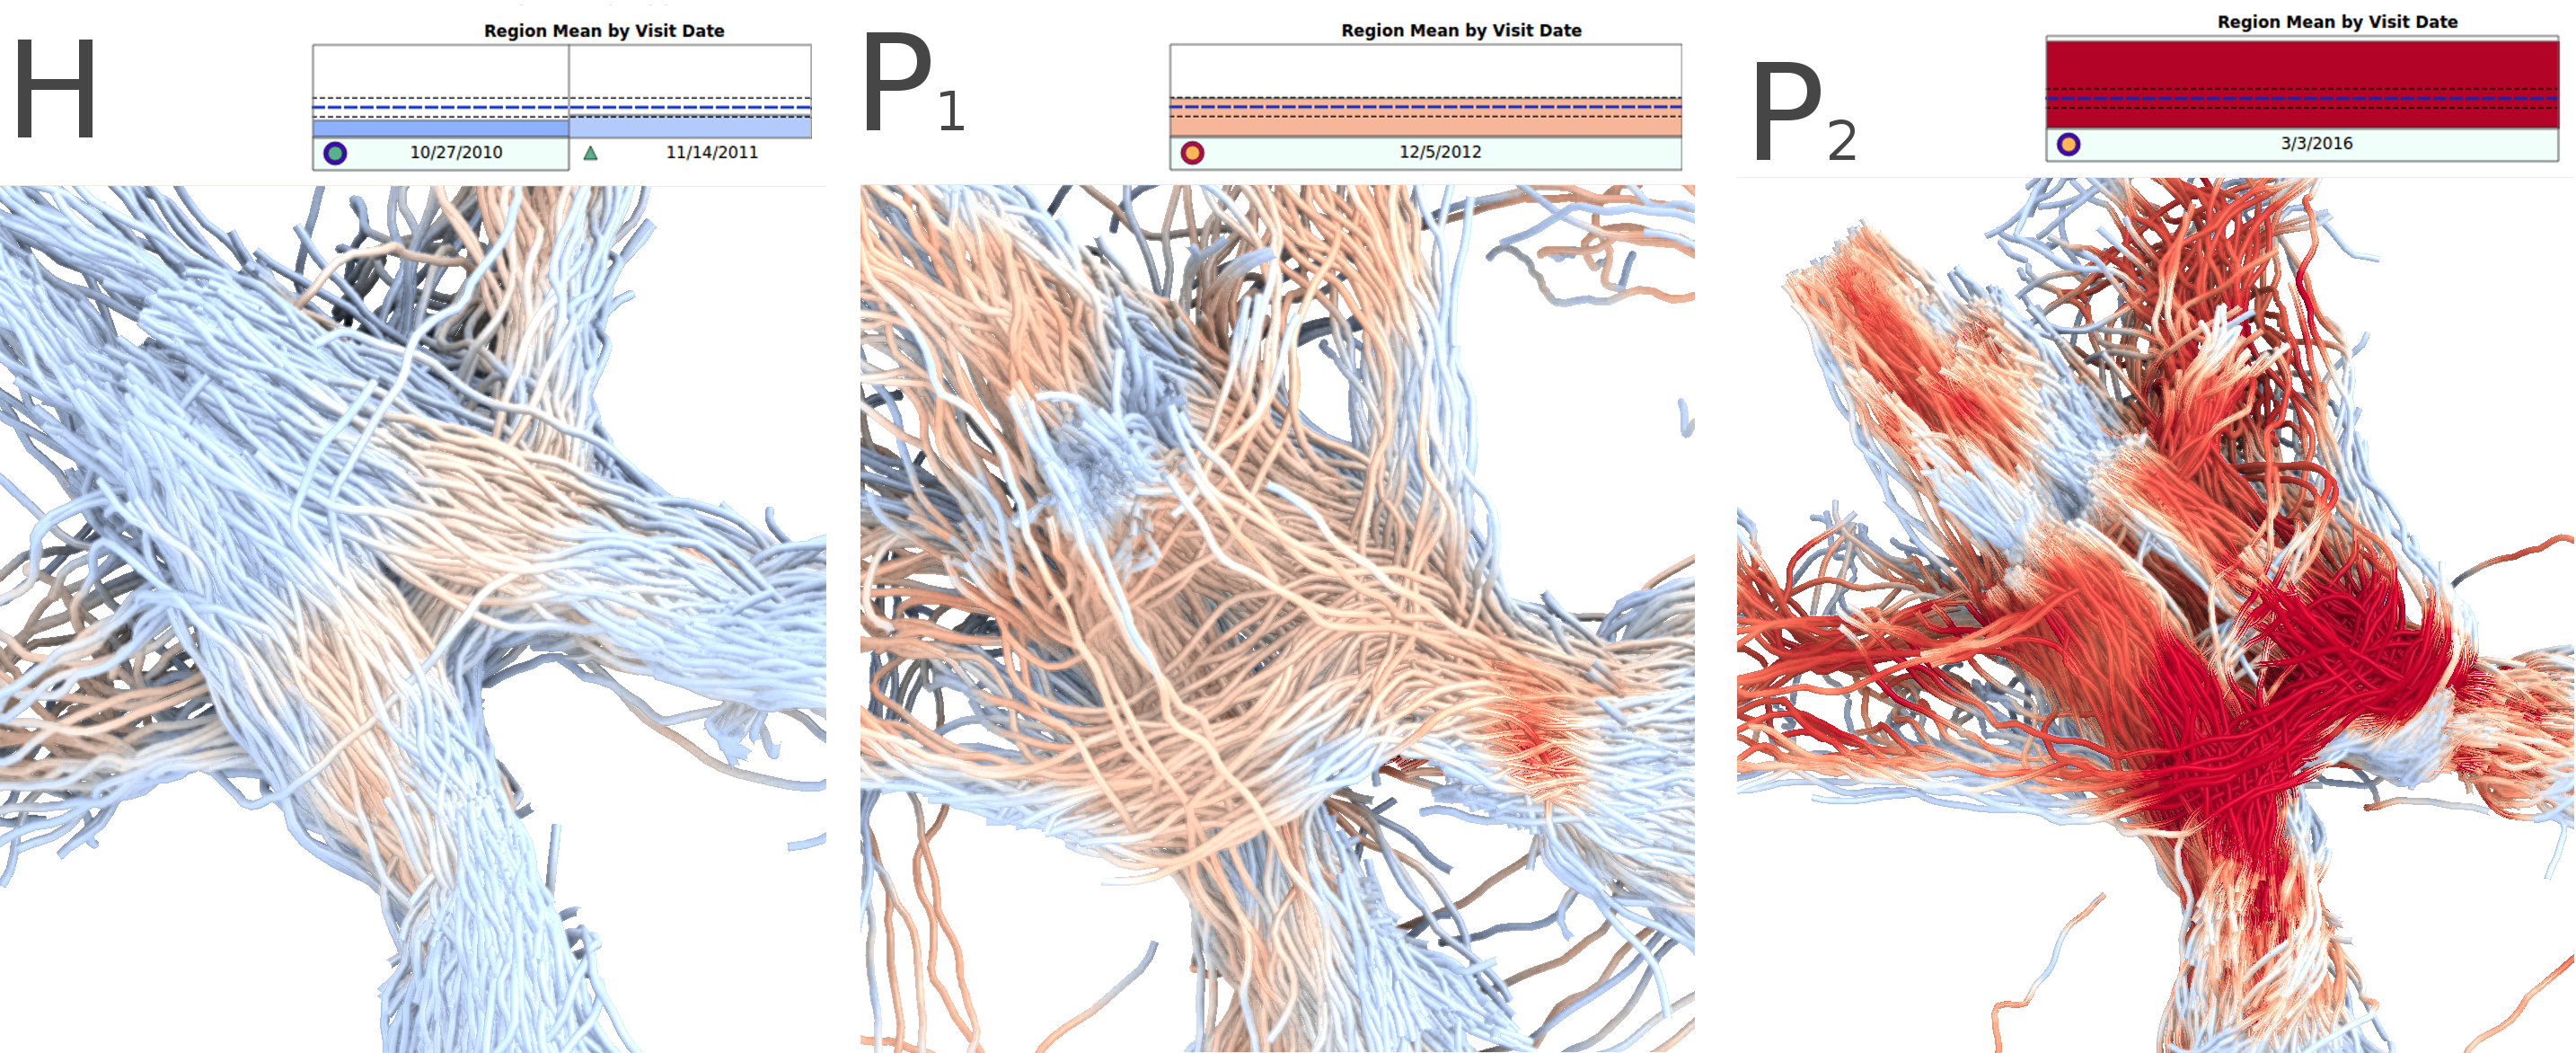
\includegraphics[width=0.5\textwidth]{SSO.png}
\caption{The substantia nigra region is rendered with the S0 feature (raw T2 signal with no diffusion weighting) mapped using color. In the top $(H)$, the region is for a control subject that has overall lower values, and is without patches. This characteristic seemed more prevalent within the control group, yet many disease group subjects have this characteristic as well. The next two images $(P_1, P_2)$ each show brains fiber tracts from the disease group. In the middle $(P_1)$, patches of high values are observed in areas near the mid-section of the region. This characteristic seemed more prevalent in the disease group, yet is also found in many control group subjects as well. In the bottom ($P_2$), an example of a subject with abnormally high signal values throughout the mid-section and outer sections of the region. This effect seemed more prominent in more disease group subjects, yet was observed in some control group subjects as well.}
\label{fig:SSO}
\end{figure}


\begin{figure}[!ht]
\centering
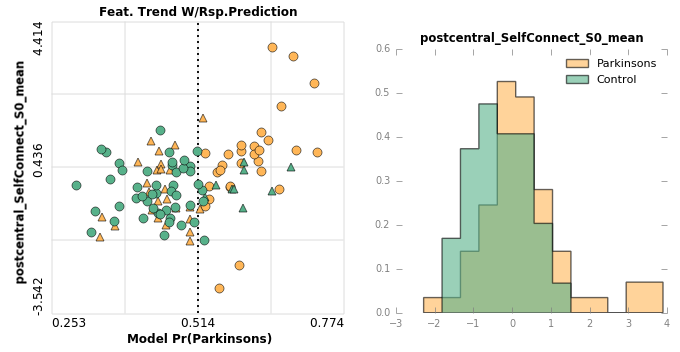
\includegraphics[width=0.5\textwidth]{PMSO.png}
\caption{Comparing the distributions of the S0 feature (raw T2 signal with no diffusion weighting) between the control group (blue-green) and disease group (orange). The disease group's distribution is centering at a higher value than the control group and there are multiple outliers from the disease group in the high value range.}
\label{fig:PMSO}
\end{figure}

\subsubsection{The Substantial Nigra Region (SN)}

\textsl{Fiber Reduction}

Based on findings from previous works, we expected to see substantial fiber loss in the Substantial Nigra (SN) region. We also expected to get high predictions using only the SN region, and that the sum or average fiber lengths in the region would be good predictors. While we did see that average fiber length was a top scoring feature for the region, and that multiple Parkinson's subjects had high loss of fibers in the expected regions, these effects were not consistent across all of the subjects, and overall there is a large amount of overlap in the distributions of these features between the control and disease groups. One of the most significant features capturing the effect of fiber loss in the region seemed to be the absolute difference between the sum of the fiber lengths in the left hemisphere and right hemisphere (DSFL). Figure~\ref{fig:DSFL} shows the distribution and scatter plot of the subjects average values over their predicted probabilities. Figure~\ref{fig:loss} shows the type of loss we found in some of the Parkinson's brain fiber tracts in the SN region. The leftmost image shows a typical fully intact region for a control subject, while the right three images show progressively worse cases of fiber loss. The coloring shows the difference in the length of the fiber from the average length of the control groups fibers for this region.

\textsl{ Raw T2 signal with no diffusion weighting (S0) } 

One of the top ranked features for the SN region was the raw T2 signal with no diffusion weighting (S0) feature. While ranked as one of best features, there was still a large overlap between the disease and healthy control groups, and the overall predictive power of the feature was still quite poor. By investigating the feature in the physical fiber rendering views with the values mapped to each point in each fiber, we were able to see some interesting trends and features. The trends that we found are shown in Figure~\ref{fig:SSO}. The first is overall lower values, and less intense local values, which seams more typical of control group fiber tracts. The second is the occurrence of patches of high S0 values occurring near the mid-section of the SN region (near the center), as seen the red spot in P1 image of Figure~\ref{fig:SSO}. While this seemed more typical of the disease group subjects, this effect was also noticed in many control group fiber tracts. The last is characterized by very high intensities in the mid-section and mid-outer reaches of the fibers. This effect was noticed also in both groups, but seemed more typical of the Parkinson's group. One interesting subject in particular is a 77 year old female with Parkinson's disease who has very complete fibers in the SN region. However, our classification models consistently predicted her to have Parkinson's with high confidence ($>90\%$ probability). After visualizing S0 mapped to the SN region fibers, we found she was an outlier in this feature with very high intensity values, likely this accounts for her high probability prediction.

\begin{figure}[!ht]
\centering
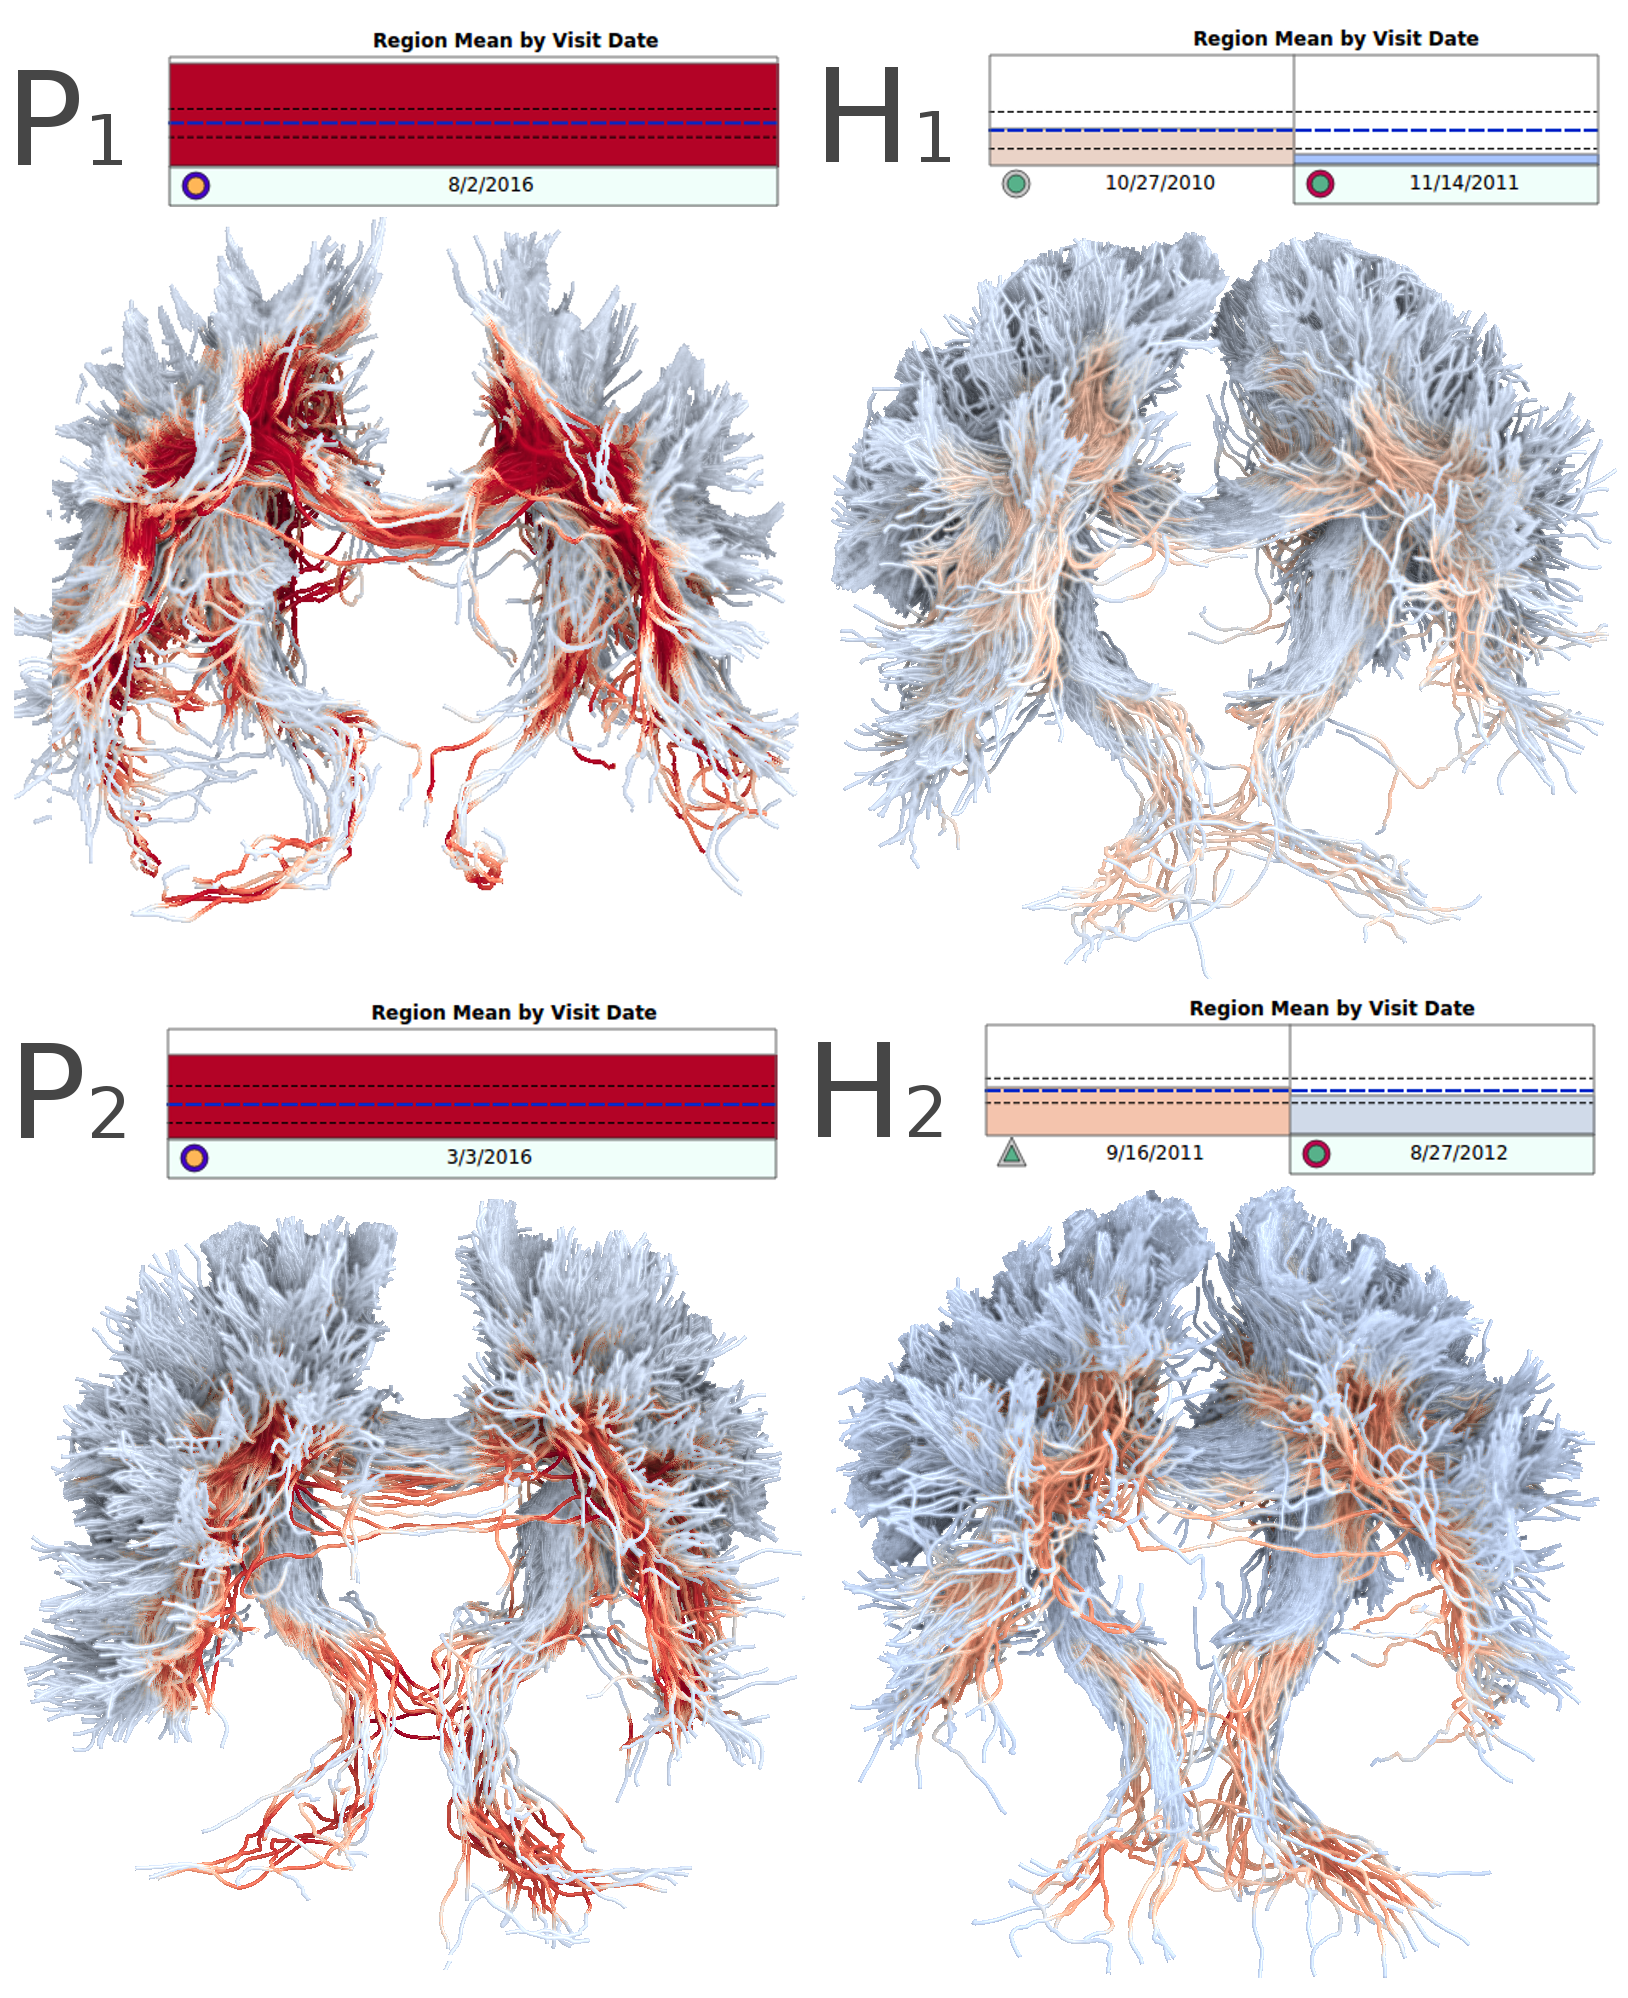
\includegraphics[width=0.5\textwidth]{pregion.png}
\caption{Some examples mapping the Raw T2 signal with no diffusion weighting (S0) to the Post Central Region. On the left column we show two subjects from the disease group with a noticeable trend that we found to be mildly more prevalent in the disease group. On the right side we show two control group subjects for comparison.}
\label{fig:pregion}
\end{figure}

\subsection{Effects of Parkinson's on the Post Central Region}

One of the top ranked region for prediction was the Post Central region. The highest ranked feature within the region was the raw T2 signal with no diffusion weighting (S0). The distribution and scatter plot is shown in 
Figure~\ref{fig:PMSO}. We investigated the feature values on the fibers in the physical space and found a trend similar to the trend we found for this feature in the SN region. Overall, it seams that the Parkinson's group shows more subjects with higher values in the inner section of the region. Several images of the fiber rendering for this case are shown in Figure~\ref{fig:pregion}.

\section{Discussion}

Our work addresses an important challenge in the study of the effects of neurodegenerative diseases on the human brain. While our design brings together the primary stages of the typical machine learning pipeline into a synergistic visual analytic system, there are several ways in which one could extend our work to gain additional benefit.

While the user is investigating the physical manifestations underlying statistical features, they may find some useful insights for creating new features that are better able to predict the disease. For example, we observed in our case studies that the differences between the control group and the healthy group can be subtle, and localized, or dispersed, causing the summary statistic to be too `watered down'' to effectively distinguish the two groups. One remaining challenge would be to integrate more advanced feature extraction techniques or develop new ones which are better able to localize and capture the effects of the disease. Several previous works\cite{dinov2016predictive, zhang2015detection, plant2010automated} noted in our related works section may be good candidates for future experimentation and engineering. 

Another direction for future improvement is to aid the user in finding these types of localized and or dispersed physical features in the visualization. While our rendering methods and color mapping highlight these features effectively, occlusion can still cause some of them to be hidden in the interior of fiber bundles. We also noted some works\cite{jianu2009exploring,jianu2012exploring} that we mention in our related works section that address this type of challenge by studying the ways in which fibers can be projected into a 2D or 3D space as points. If one could project the fibers into a 2D space while maintaining the ability to see its connections and prevent occlusion as best as possible, it might help to better show these features, and select the corresponding fibers. Another approach could be strategic use of transparency along with view point optimization. One challenge is the difficulty in defining the feature of interest when there can be many differences and variations of same effect over different subjects.

Also, several works have addressed uncertainty visualization in DTI fiber tracts. Our system implicitly addresses uncertainty to an extent, through significance testing of the features between groups, predictive performance, and visual comparison of multiple subjects over different scans. Still it could be beneficial to incorporate some uncertainty visualization of the DTI tensors themselves directly.

While we used about $30$ days worth processing time to reconstruct the fiber tracts and connectomes from the $~120$ brain images we acquired, we feel that this number is still too low to train a reliable enough model to use in practice. While we stratified our selection of $DTI$ images by age and group, we believe that the number of same age patients in each age group is too low with this number to properly deal with this confounding factor. Additionally, it would be beneficial to have more scans to better stratify as well by gender. Although many more DTI images can be found at PPMI, the processing time is expensive. 

Finally, we would like to make our system available to be used for medical research, and hope to develop a deeper collaboration with neuroscientists studying neurodegenerative diseases, including both Parkinson's and Alzheimer's as a starting point.